\documentclass[a4paper,12pt]{report} 

   \setlength{\textwidth}{6.25in} % original 6.25
\setlength{\textheight}{650pt}
\renewcommand{\baselinestretch}{1.3}

\oddsidemargin 20pt    %  Left margin on odd-numbered pages.
\evensidemargin 20pt   %  Note that \oddsidemargin = \evensidemargin
\topmargin 0pt
\thispagestyle{empty}
\pagestyle{empty}
\fontencoding{T1}
\fontfamily{times-tt}
\rmfamily
\usepackage{amsmath} 
\usepackage {graphics}
\usepackage {epsfig}
\usepackage {graphicx}
\usepackage {fancyhdr}
\usepackage{epstopdf}
\usepackage[final]{pdfpages}
\usepackage[left=1.50in,top=1.0in,bottom=1.0in,right=1.0in]{geometry}
\usepackage {fancyheadings}

\usepackage[]{hyperref}
\usepackage{tikz}

\usepackage{tabularx}

\usepackage[nottoc,notlot,notlof,numbib]{tocbibind}
\usepackage[titletoc]{appendix}
\usepackage{titletoc}
\renewcommand{\appendixname}{Annexure}
\renewcommand{\bibname}{References}

\setcounter{secnumdepth}{5}

\usepackage{float}
\usepackage{subcaption}
\usepackage{multirow}

\usepackage[ruled,vlined]{algorithm2e}


\begin{document}

\begin{center}
\noindent \large\textbf A 

\noindent \large \textbf { PROJECT REPORT}

\noindent \textbf { ON}

\noindent \textbf{``A Real Time Flood Monitoring System and Warning System Via Social Media using IoT and Wireless Networks"}


\noindent \textbf{}

\noindent\large
SUBMITTED TO THE SAVITRIBAI PHULE PUNE UNIVERSITY, PUNE, IN THE PARTIAL FULFILMENT FOR THE AWARD OF THE DEGREE OF

\hspace{0.1in} 

\noindent\large\textbf{BACHLOER OF ENGINEERING}

\textbf{ Computer Engineering}



\noindent \large SUBMITTED BY

\noindent \textbf{}
\noindent {\textbf{Mr. Mayur Tajane  \hspace{35 mm}         B}}\\
\noindent {\textbf{Mr. Harshal Chaudhari  \hspace{21 mm}	B}}\\
\noindent {\textbf{Ms. Monali Sonawane \hspace{25 mm}    B}}\\ 
\noindent {\textbf{Ms. Mayuri Sonavane     \hspace{24 mm}     B  }}\\


\newline
\vspace{0.2in}
\large{\textbf{ UNDER THE GUIDANCE OF}} 

\large{\it Prof. J.Y. Kapadnis }

\noindent \textbf{}
\begin{figure}[tph!]
\center {\includegraphics[totalheight=2.5cm]{logo.png}}
  
    \label{fig:verticalcell}
\end{figure}

\noindent \large\textbf{DEPARTMENT OF COMPUTER ENGINEERING}
\noindent \textbf{
\newline Pune Vidyarthi Griha's College of Engineering,}
\noindent \large\textbf{\newline Near MERI, Dindori Road, Nashik-422004}\\
\large\textbf{ ACADEMIC YEAR 2019-20 }
\textbf{}
\end{center}
\newpage
%\newpage
%\noindent \textbf{ }
\noindent \textbf{}


{\bfseries \fontsize{16}{12} \selectfont \centerline{CERTIFICATE} 
\vspace*{3\baselineskip}} 

\centerline{This is to certify that the Project Entitled}
\vspace*{1\baselineskip} 

\textbf{A Real Time Flood Monitoring System and Warning System Via Social Media using IoT and Wireless Networks}

\vspace*{1\baselineskip}}

\centerline{Submitted by}
\begin{center}

\noindent {\textbf{Mr. Mayur Tajane  \hspace{33 mm}         B}}\\
\noindent {\textbf{Mr. Harshal Chaudhari  \hspace{21 mm}	B}}\\
\noindent {\textbf{Ms. Monali Sonawane \hspace{25 mm}    B}}\\ 
\noindent {\textbf{Ms. Mayuri Sonavane     \hspace{24 mm}     B  }}\\
\end{center}
is a bonafide work carried out by them under the supervision of  Prof. J.Y. Kapadnis and it is approved for the partial fulfillment of the requirement of  Savitribai  Phule Pune University for the award of the Degree of Bachelor of Engineering (Computer Engineering).
This project report has not been earlier submitted to any other Institute or University for the award of any degree or diploma.\\\\
\large{}\hspace*{1.5in}\large{}\large{}\\[0.2cm]
Prof. J.Y. Kapadnis \hspace{1.5in} Prof. J.Y. Kapadnis\\
{Internal Guide} \hspace{1.7in}{HOD, Computer Engineering Dept}\\
\large{}\hspace*{1.5in}\large{}\large{}\\[0.2cm]\\
Seal of College\hspace{1.9in}Principal\\
\large{}\hspace*{0.6in}\large{}\large{}\\[0.2cm]
Place: \hspace{1.9in} \\
Date:\hspace{0.7in}\\
\large{}\hspace*{1.5in}\large{}\large{}\\[0.3cm]





\newpage
%\frontmatter
%\noindent \textbf{}
\vspace{2cm}
\pagenumbering{roman}
\addcontentsline{toc}{chapter}{Acknowledgement}
\begin{center}
\LARGE\bf{Acknowledgement}
\end{center}
\vspace{1in}

We sincerely express our deep sense of gratitude towards our respected guide and head of department\textbf{ Prof. J.Y. Kapadnis} for his valuable guidance, profound advice, persistent encouragement and help during the completion of this work. His time to time helpful suggestions boosted us to complete this task successfully. He has helped us in all possible ways right from gathering the materials to report preparation. We express our thanks to our guide and Project coordinator for providing all kinds of co-operation during the course. Our sincere thanks to the Principal \textbf{Dr.Edlabadkar Sir} for his inspiration. Finally, we are thankful to the supporting staff of Computer Engineering department and all those who directly or indirectly contributed to complete this work. We sincerely thank you to our project co-ordinator Prof. M.T. Jagtap for guiding us.



\noindent \textbf{}

\begin{center}
\noindent {\textbf{Mr. Mayur Tajane  \hspace{35 mm}         B}}\\
\noindent {\textbf{Mr. Harshal Chaudhari  \hspace{21 mm}	B}}\\
\noindent {\textbf{Ms. Monali Sonawane \hspace{25 mm}    B}}\\ 
\noindent {\textbf{Ms. Mayuri Sonavane     \hspace{24 mm}     B  }}\\
\end{center}
\clearpage



\begin{center}
\pagenumbering{arabic}
\noindent\LARGE \textbf{Abstract}
\end{center} 
\newline
Flood is the most significant disaster happened in
almost every part of the world. When the event occurred, it
causes great losses in economic and human life. Implementation
of the advancement of ICT brings significant contribution to
reduce the impact of flood toward the people and properties.
This paper attempts to investigate the capability of internet of
things (IoT) technology in reducing the impact of natural
disaster specifically in flood disaster scenario. First, the concept
of Internet of Things (IoT), key technologies and its architecture
are discussed. Second, related research work on IoT in disaster
context will be discussed. Third, further discussion on the
propose Internet of Things (IoT) architecture and key
components in the development of flood prediction and early
warning system. The smart sensors will be placed at river basin
for real-time data collection on flood related parameter such as
rainfall, river flaw, water level, temperature, wind direction and
so on. The data will be transmitted to data centre via wireless
communication technology which will be processed and
measured on the cloud service, then the alert information will be
sent users via smart phone. Thus, early warning message is
received by the people in terms of location, time and other
parameters relate to flood.\\
\textbf{Keywords:-} \textit {flood,dissaster management, nodemcu, social media alerts, ultrasonic sensor, mqtt.}



\noindent ~

\newpage
%\frontmatter
%\noindent \textbf{}
\vspace{2cm}
\pagenumbering{roman}
\addcontentsline{toc}{chapter}{Abstract}

\tableofcontents




\noindent

\newpage
\listoffigures
\noindent

\noindent \textbf{}
\noindent








\noindent
\newpage

%\pagenumbering{arabic}
\large

\pagestyle{fancy}

\lhead{}

\chead{A Real Time Flood Monitoring System and Warning System Via Social Media using IoT and Wireless Networks  }

\rhead{\thepage}


\fancyfoot[CO]{PVGCOE,Nashik-Computer Engineering.}

\fancyfoot[CE]{PVGCOE,Nashik-Computer Engineering.}
\pagenumbering{arabic}

\vspace{0.1in}
\vspace{0.1in}


\chapter {Introduction}
Flood is the biggest natural disaster happens in worldwide without prior warning. Floods will damage the crops, cars, buildings, homes and anyone in their path. Reservoir is the most efficient tool to save the water resource; Reservoirs are serving for different purposes in spatial and temporal method such as a hydropower generation, flood control, navigation, ecology and recreation. The flood-limited water level (FLWL), is the parameter to manage between the flood control and conservation, from that the annual maximum value is determined. It is done mainly according to design flood estimation flood series, while it neglects seasonal flood information. At present, many research works on IoT in disaster domain have been conducted. This section will provide a summary on research works that implement IoT technologies for addressing natural disasters. IoT technologies give benefits in terms of monitoring, tracking, controlling and sensing the 

environment using real time data. The use of IoT to improve environmental monitoring and management tasks. The results from their case study demonstrate that the Integrated Information System (IIS) based on IoT is valuable and efficient for complex tasks in environmental monitoring and management. The use of IoT technologies in tackling the complexity in monitoring the flood specifically using rain gauges. IoT provides an interface for data streaming management in real time and at the back end provide data analysis and visualization. In this approach the data collected will be continuously transmitted via the Internet communication infrastructure, to the software components. The software components are designed to compute the stream flow and to quantify the spatial distribution of flood risk for each controlled watershed. The use of IoT and machine learning based embedded system to predict the probability of floods in a river basin. To develop A Real Time Solution to Flood Monitoring Using IoT and Wireless Sensor Network, we proposed a flood warning system which requires attention to three basic factors: Data collection via gaging, data processing, and the hardware and software required, and the dissemination of flood warning information. While automated flood warning systems are often surprisingly inexpensive to implement, the primary factor determining cost for any such system is the number of gage site locations. Severe flooding affected Indian state of Kerala due to unusual high rain during monsoon season. It was the worst flooding in Kerala in nearly a century. In which over 373 people died within fortnight. Thirty-five out of 42 dams within the state open for the first time in history. Kerala received heavy monsoon rainfall on the midevening of August and resulting in dams filling to capacity in the first 24 hours of rainfall the state received 310 mm of rain.
 

\section{Motivation}
In the current year i.e. 2019 maharashtra and kerala states faces several flood situations; in which many districts and millions were affected by the flood. Kolhapur , Pune and Nashik district mainly faces flood situation during the July, august and September month.    Millions were affected by the situation. So many lost their lives and day to day life is disturbed and destroyed.
This can be overcome by providing early warning of upcoming disaster by using available resources.   Our main aim of this proposed system is to avoid upcoming disastrous situation by alerting those people who are going to face such situation.
The People who faces flood situation mostly located nearby river bank. In the current year nashik mega flood level raised up to 25 to 30 feet. In Kolhapur district most of rural and urban areas were underwater.


\section{Problem Definition}
To design and develop a real time system that sense rising water level of river basin by using sensors which is going to transfer and store to database ; and as per condition a warning message is going to deliver to those people who’s going affected by such situation.



\chapter {Literature Survey}
\textbf{[1] DIAO YanFang WANG BenDe ,Risk analysis of flood
control operation mode with forecast information based
on a combination of risk sources.Sci.China Tech.
Sci. MAY 2008.}\\
Flood Control Operation Mode with forecast information (FCOMFI) is an important base for risk analysis
of the reservoirsDIAO YanFang\& WANG BenDe have analyzed the four uncertainties that is hydraulic, hydrological,
stage-storage uncertainty and time-delay uncertainty, and also their probability distributions. This proposed model was
estimate by Monte Carlo simulation, based on Latin hypercube sampling. The major potential risks are includes in two
methods i. Risk of reservoir ii. Risk of lower reach. Monte Carlo simulation is a statistical sampling technique that
generates random variables that preserve the distributional properties and provide numerical evaluations of the
probabilistic features of the system response. The risk analysis of FCOMFI aims at the safety of the reservoir and the
effective utilization of the flood water resources.
\textbf{[2]Ruan Yun, Vijay P. Singh ,2008, Multiple duration lim-
ited water level and dynamic limited water level for
flood control, with implications on water supply, (2008) }\\
 Flood control, which may be equally important in semi-arid areas, correspond to two different reservoir
water levels. The first is the limited water level it can be used for flood control. There are two approaches are proposed
byRuan Yun, Vijay P. Singh ,one is multiple duration limited water level and second is dynamic limited water level.
This paper also proposed a dynamic limited water level for flood control build on conditional probabilities of large
storms. This means that the annual limited water level for the flood season can be modified by the several multiple
duration limited water levels such as monthly duration limited water levels or weekly duration limited water levels.\\
\textbf{[3]HEIKO APEL, ANNEGRET H. THIEKEN, BRUNO
MERZ andGU NTER BLO SCHL, A Proba-
bilistic Modelling System for Assessing Flood Risks,2016}\\
 Flood disaster mitigation based on a comprehensive assessment of the flood risk. ‘‘German Research
Network Natural Disasters’’ project, the working group on ‘‘Flood Risk Analysis’’ searching complete flood disaster
chain from the triggering event down to its various consequences. The ‘‘Flood Risk Analysis’’ group developed
complex, spatially distributed models. It represent the relevant hydrological, hydraulic, meteorological, geo-technical,
and socio-economic processes. The flood disaster chain represents the two way approaches (simple probabilistic and
complex deterministic). This approach allows the various number of simulation runs in a Monte Carlo framework and
provides the support for a probabilistic risk assessment. The proposed model is useful to integrated assessment of flood
risk in flood prone area.. Applying this concept, it is the most important failure mechanism for new river levees. The
breach criterion is scope as the difference between the actual overflow and the critical overflow.All modules are
combined in a Monte Carlo framework. First, a discharge value was randomly chosen from the composite flood
frequency. Second flood type was randomly chosen.\\
\textbf{[4]BastianKlein,MarkusPahlow,
Yeshewatesfav Hundecha and Andreas
Schumann, 2005,Probability Analysis of Hydrological
Loads for the Design of Flood Control Systems Using
Copulas.J. Hydrol. Eng}\\
 The risk analysis of a flood control system is presenting a method, to estimate the probability of generated
hydrological scenarios. Using copulas bivariate probability analyses of different flood variables are applied univariate
probability to overcome that analysis may lead to an over- or underestimation of the hydrological risk. Which consists
of two reservoirs located downstream of the main tributaries and flood polders. The joint probability of the inflow
peaks at the two reservoirs are analysed the spatial distribution of flood events within the river basin. Risk analysis of
the individual flood detention structures are use in second application copulas.
Recent researches in flood prediction depict the use of
wireless sensor networks and advanced artificial neural
networks. \\
\textbf{[5]Simon Haykin, Neural Networks A Comprehiensive
Approach.}\\ 
Seal et al. have utilized a wireless sensor network
(WSN) to collect data and used a linear regression model with
multiple variables for real-time and accurate flood prediction
results. Increase in water level indicates flood if it exceeds the
flood line. \\
\textbf{[6]V. Seal, A. Raha, S. Maity, S. Mitra, A. Mukherjee and
M. Kanti Naskar, A Simple Flood Forecasting Scheme
Using Wireless Sensor Networks, 2012.}\\
 Furquim et al. have also utilized WSN and various
types of machine learning classification techniques for flash
flood nowcasting. They have made a comparison of the
performance of these techniques with different data
representations. The multilayer perceptron technique has shown
better results in their work. However, some of the used sensors
have not been tested in their work.\\
\textbf{[7] G. Furquim, F. Neto, G. Pessin, Jo Ueyama, J. P. De
Albuquerque, Combining Wireless Sensor Networks and Ma-
chine Learning for Flash Flood Nowcasting, IEEE, 2014.}\\
Nuhu et al. have utilized 6 Low power Wireless Personal
Area Network (6LoWPAN) as a communication technology
with the help of XM1000 motes for real-time flood monitoring.
A water level monitoring is done based on pre-defined rule
based system. Though the system shows good accuracy with
lower power consumption, the cost of motes in the work is very
high. \\
\textbf{[8]B. Kontagora Nuhu, T. Arulogun, I. Adeyanju and Ab-
dullahi I.M., Wireless Sensor Network for Real-time
Flood Monitoring Based on WPAN Communication
Standard, 2016.}\\
 Ancona et al. have discussed an IoT approach for flood
monitoring using highly dense grid of rainfall sensors and river
gauges to measure water level. It also discusses about the
integration of sensors’ infrastructure with various IoT cloud
platforms. It also speaks of development of ultra-low power
sensors or devices for the purpose.\\

\textbf{[9]S. Gangopadhyay and M. Mondal, A Wireless Frame-
work for Environmental Monitoring and Instant Re-
sponse Alert, 2016.}
\\ Gangopadhyay et al. have implemented wireless IoT
framework using Arduino Uno and an array of sensors
connected to it. They utilize Xbee transceivers for
communication and upload the data on ThingSpeak and Xively
cloud servers. Their experiment shows that ThingSpeak is a
better IoT cloud platform for this purpose. Also an instant alert
is sent to the users through Twitter or the android app developed.
However the system cannot accurately predict the event of flood
in their work as they have not deployed a model for it. [10] Mitra
et al. have proposed an IoT based WSN system for flood
forecasting purpose. They have used Zigbee technology for
communication between nodes and CC2650 MCU as a central
controller. For communication over internet they have made use
of GPRS Sim300 module. Further they have proposed use of
simple ANN structure with five input parameters and water level
as output. They have simulated the entire system and tested
ANN model on old satellite data. They have not yet practically
implemented the system and have also not used the real-time
WSN data for prediction purpose. Also no alert system is
developed.\\
\textbf{[10]P. Mitra, R. Ray, R. Chatterjee, R. Basu, P. Saha,
S. Raha, R. Barman, S. Patra, S. Saha Biswas and Saha, Flood forecasting using Internet of things and Artificial Neural Networks, 
2016.}\\
 S. Ruslan et. al. have proposed Nonlinear Auto Regressive
with Exogenous Input (NARX) model to mitigate the problem of
nonlinear flood prediction problem. The system predicts the
occurrence of flood in Kelang River with a lead-time of 10
hours.
In this work, we have developed a ultra low power IoT flood
monitoring system using low-power sensors and a dashboard
developed by ThingSpeak is used to depict the real-time data
collected by the system. The ANN flood prediction model is
implemented on the real-time collected data and the prediction
of flood event is done. Also an alert system is proposed based on
the ThingSpeak messages on registered Twitter accounts. 



\chapter {Software Requirement Specification}
\section{Introduction}
\subsection{Project Scope}
This flood alert system is basically useful to get idea about flood in forecast to do the sensing of the incoming water level for detection of flood is done by implementing sensors. In this way water level will be sensed by the sensor and concerned messages will be given to the controller then it will take the further action on that command.





\subsection{User Classes and Characteristics}
\textbf{1. User:- }\\The user is the authority will monitor the system by using the website. The system will notify the user using text and mails. The user is may be the municipalty officer or any other higher authority who will maintain the sewage system of the city. \\ 
\textbf{2. NodeMCU:-}\\ NodeMCU is an open source IoT platform. It includes firmware which runs on the ESP8266 Wi-Fi SoC from Espressif Systems, and hardware which is based on the ESP-12 module. The term "NodeMCU" by default refers to the firmware rather than the development kits. The firmware uses the Lua scripting language. It is based on the eLua project, and built on the Espressif Non-OS SDK for ESP8266. It uses many open source projects. \\\newline
\textbf{3.Cloud System:-}\\ The Cloud system is storage where we can store our data coming from sensors like ultrasonic sensor and water level sensor. The cloud system will display the readings using the website. \\\newline
\textbf{4. Sensors:-}\\ The sensors will play the main role in this system. The sensors include the ultrasonic and water level sensor which will read the input coming from the drainage system and send this readings to nodeMCU.  

\subsection{Assumptions and Dependencies}
1. Assume that laborotory is equiped with all facilties. \\
2. We assume that user knows how to operate system. \\


\section{Functional Requirements}
\textbf{1. Administrative functions:-} \\
This system should provide the administrative functions like registration and login for normal users.\\
\textbf{2. Authentication:-} \\
Thr proposed system authenticate user by their username and password for security reasons.\\\newline
\textbf{3. External Interfaces:-} \\
The system should provide the interface to other systems for external system for better performance. \\
\textbf{4. Historical Data:-} \\
For performance improvement we have to store the historical data of the system so that we can compare the performance of system. \\

\section{Extrenal Interface Requirements}
\subsection{User Interfaces}
The web based application is used to communicate with the system.
\subsection{Hardware Interface}
The computer system is used to control the system. 
\subsection{Software Interface}
We need the Textlocal API for the text message alerts for users. 
\subsection{Communication Interface}
The http protocol is used as communication protocol for this system.
\section{Nonfunctional Requirements}
\subsection{Performance Requirements}
The system should have a high throughput.It should handle
complexity. The response time of the system should be mini-
mum. System must be user friendly so, that user interaction will
be smooth and efficiency increases.sample user logs should be
analyzed properly. system classification should be done prop-
erly in less amount of time.system recommendation should be
accurate enough that satisfy the user.
\subsection{Safety Requirements}
The system should have a high throughput.It should handle
complexity. The response time of the system should be minimum. System must be user friendly so, that user interaction will
be smooth and efficiency increases.sample user logs should be
analyzed properly. System classification should be done properly in less amount of time.system recommendation should be
accurate enough that satisfy the user.
\subsection{Security Requirements}
1. Working must be in formatted way. \\
2. No losses or causes due to the use of this system. \\
\subsection{Software Quality Requirements}
\textbf{1. Adaptability:}\\ Proposed System can be adapted easily to various
operating environments. \\\newline
\textbf{2. Availability:}\\ Can easily execute on currently available minimum
configuration of hardware and software. \\\newline
\textbf{3. Correctness:}\\ It will work correctly according to the valid input
requirements. \\\newline
\textbf{4. Usability:}\\ This system used in different mobile phones or any
device. \\
\section{System Requirements}

\subsection{Databse Requirements}
The database required in this system is stored on the cloud. We store
the historical data on cloud for future use.

\subsection{Software Requirements }
\begin{itemize}
\item  Ardiuno IDE
\item  Google API
\item  Textlocal API
\item  Php Myadmin
\item  HTML,CSS
\end{itemize}

\subsection{Hardware Requirements}
\begin{itemize}
\item  NodeMCU ESP8266 12E
\item  Ultrasonic Sensor
\item  Water Level Sensor
\item  Water Flow Sensor
\item  Temp Sesnor
\end{itemize}


\chapter {System Design}
\section{System Architecture}


\begin{figure}[H]
  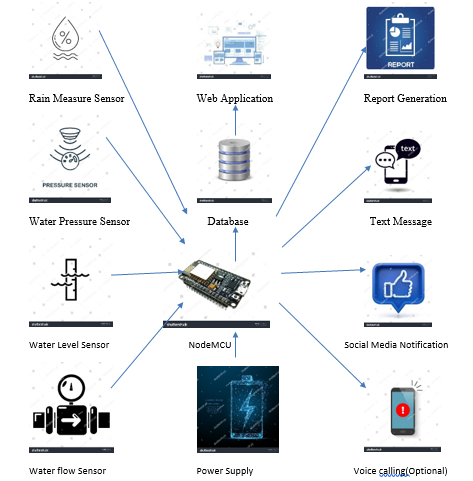
\includegraphics[width=5 in]{d1.png}
  \caption{System Architecture}
  \label{fig:boat1}
\end{figure}


1. There will be a node as shown in above diagram. \\
2. This node is the independent flood monitoring node equipped with necessary sensors and connectivity modules. \\
3. It has three major stages, Including Sensors, Controller, Wi-Fi interface to upload the information on server.\\
 4. Data from various sensors are collected by the ESP and is then computed and uploaded on the server.\\
 5. The data uploaded on server is stored on the database. \\
6. The stored data is then routed to the front end web applications and mobile applications.\\
\section{Working of the Proposed System}
IoT technologies give benefits in terms of monitoring, tracking, controlling and sensing the environment using real time data. An introduction of the use of IoT to improve environmental monitoring and management tasks [11]. The results from their case study demonstrate that the Integrated Information System (IIS) based on IoT is valuable and efficient for complex tasks in environmental monitoring and management. The use of IoT technologies in tackling the complexity in monitoring the flood specifically using rain gauges [12]. IoT provides an interface for data streaming management in real time and at the back end provide data analysis. In this approach the data collected will be continuously transmitted via the Internet communication infrastructure, to the software components. The software components are designed to compute the stream flow and to quantify the spatial distribution of flood risk. Use of IoT and machine learning based embedded system to predict the probability of floods in a river basin.\\

Some Features we are going to implement in the proposed system are as follows: -\\
1)	We are doing continuous monitoring of the river water level and record its data into relevant database.\\
2)	Also we are monitoring the water level of the dam which is concerned with that particular region or provinces.\\
3)	If due to heavy rain fall into that particular region or continuous rain into that region the administration authority release or discharge the water from the dam (Measures mostly in Cusec and Cumec); Then with the help of proposed system, we can calculate approximate level that is going to up rise into normal water level.\\
4)	When heavy quantity of water discharged from the dam at that time warning message will be delivered to those people who having residence nearby river bank as well as the government authority who is responsible for help and relieve duties like municipal corporation and fire and rescue department.\\
5)	If a consider a situation where a flood zone having active electricity supply or the flood water contains high voltage electricity (greater than 440 volts A.C.) then we deliver a message to the victims as well as the help and rescue department along with the local government like municipal corporation.\\
6)	An advance module we are going to add into proposed system is that we are going to collect acknowledgement from the victims or the people to them we are going to deliver the warning message. Acknowledgement is collected by receiving and measuring the reply message that we have broadcasted. By comparing both data we an easy find out who is trapped into and need evacuation and help.\\
7)	This acknowledgement report is going to submit to government authorities to help them start them relieve operation for the flood victims.\\
8)	An additional module is going to add is to detect land movement to nearby to high climbed or ridge zones to detect landslides. This used to help rescue lives before such disaster occur. Each city contains such kind of zones which needs to monitor on continuous basis. In heavy rainfalls landslides can be occur without any kind of warning and causes very big impact in the form of lives and wealth casualties.\\
9)	If water increases rapidly and it is going higher than he road level of the bridge or the water level goes higher than the bridge then the alert message is delivered that the particular that bridge closed for vehicles and to the government authorities as well as on the social media platforms.\\
10)	When that bridge is closed for vehicle then alter alternate road availability message is going delivered.
 

\section{Implementation Details (Modules)}
\subsection{Hardware module }
In this project, some hardware is used that are Microcontroller, sensors, components required for power supply. The Hardware collects the water level, Pressure of water, Rainfall measure to detect the levels of the flood. The hardware consists of Wi-Fi enabled controller which connects to the server and allows to share the data to through internet. \\
1. Microcontroller- This does the controlling with processing. Microcontroller will take the information from the sensor. This information will have sent to the admin through the database. \\
2. Sensors-This will collect the information from the particular nodes which are located at certain site. There are four sensors we are going to use in this project. \\
They are as follows: \\
\textbf{Water level measurement:} This sensor is used to measure the water level height. For that we are going to use Ultrasonic sensor which emits short, high frequency sound pulses at regular intervals. If they strike an object, then they are reflected back as echo signals to the sensors. \\
\textbf{Rainfall measurement:} This sensor is used to measure the average rainfall. For that we are going to use same ultrasonic sensor. Ultrasonic sensor is 4 pin sensor. Those are ground connection (GND), Trigger, echo and last current (VCC). \\
\textbf{Temperature and Humidity:} This sensor is used to measure change in atmospheric temperature and humidity. For this we are using DHT11 sensor which works on one wire protocol and gives digital output. Pressure measurement: This sensor is used to determine the atmospheric pressure. For this we are going to use BMP 180 Barometric sensor. \\
3. Power Supply- In real time we get 230v AC, in actual project we do not need this amount of power supply so we convert this AC power supply to DC power supply. \\
\subsection{Software Module}
 In this module, we have done an android application as well as the Website application for this project. Admin web page will contain and display the information like Login, Registration, Number of users registered to the app, status of the sensor, safe places near flood affected area where people can migrate and that places are shown on the Map. The Android application will be used by the users who are register. After registration the user can login with aunique username and password. And then user can access all facilities provided by application. Application is provided the information like current status of water level and temperature etc. This app contain map which are show the safe places near the user and also the current place where the user is. 
\subsection{Database Module}
 Microcontroller will send the values measured by the sensors to the server. This will contain the number of users registered to App; this will also show the safe places through the Map. The data uploaded on server is stored on the database. The stored data is then routed to the front end web applications and mobile application.

\section{Data Flow Diagrams}
\begin{figure}[H]
  \includegraphics[width=\linewidth]{p10.png}
  \caption{DFD: Level 0}
  \label{fig:boat1}
\end{figure}

\begin{figure}[H]
  \includegraphics[width=\linewidth]{p11.png}
  \caption{DFD: Level 1}
  \label{fig:boat1}
\end{figure}

\section{Use Case Diagram}
\begin{figure}[H]
  \includegraphics[width=15cm,height=19cm ]{p1.png}
  \caption{Use Case Diagram}
  \label{fig:boat1}
\end{figure}

\section{Activity Diagram}
\begin{figure}[H]
  \includegraphics[width=\linewidth]{p4.png}
  \caption{Activity Diagram}
  \label{fig:boat1}
\end{figure}

\section{Class Diagram}
\begin{figure}[H]
  \includegraphics[width=\linewidth]{p2.png}
  \caption{Class Diagram}
  \label{fig:boat1}
\end{figure}

\section{Sequence Diagram}
\begin{figure}[H]
  \includegraphics[width=\linewidth]{p3.png}
  \caption{Sequence Diagram}
  \label{fig:boat1}
\end{figure}

\section{Deployement Diagram}
\begin{figure}[H]
  \includegraphics[width=\linewidth]{p5.png}
  \caption{Deployement Diagram}
  \label{fig:boat1}
\end{figure}

\section{Component Diagram}
\begin{figure}[H]
  \includegraphics[width=\linewidth]{p5.png}
  \caption{Component Diagram}
  \label{fig:boat1}
\end{figure}

\chapter {Other Specification}
\section{Advantages}
\begin{itemize}
\item Automation of work
\item  Save the money
\item  Saves the resources
\end{itemize}


\section{Limitations}
\begin{itemize}
\item  Complex Design of Network
\item  Safety issues of sensors
\end{itemize}

\section{Applications}
1)	Municipal Corporations: - \\
The Municipal Corporation has The Emergency Response Team which faces natural and human involved disasters. By using proposed system an automated message is going to deliver to those Respond Teams to help victims.\\
2)	Fire Department: -\\
The Fire Department is responsible to help the victims who are trapped into such flood situation where they can have at least information regarding upcoming disaster which going to prevent human casualties. \\
3)	Smart City Management : -\\
If such ideas included into smart city development then it could improve the impression of that city over other cities regarding early warning relive support.


\chapter {Conclusion }
The success of flood disaster management depends largely on how well flood related data can be collected, managed and utilized. Due to this importance, the use of IoT to facilitate flood data management is seen as a step in the right direction. With the proposed architecture, future research works on flood that makes use of IoT will have a reference to specify how the work can fit within the larger flood management system.  \newline



\appendix 
\addcontentsline{toc}{chapter}{APPENDICES}


\chapter{Laboratory assignments on Project Analysis of Algorithmic Design}
\section{Introduction to IDEA Matrix:}
\begin{itemize}
\item To develop the problem under consideration and justify feasibilty using
concepts of knowledge canvas and IDEA Matrix.\\
Refer \cite{innovationbook} for IDEA Matrix and Knowledge canvas model. Case studies are given in this book. IDEA Matrix is represented in the following form. Knowledge canvas represents about identification  of opportunity for product. Feasibility is represented w.r.t. business perspective.\\ 

\begin{table}[!htbp]
\begin{center}
  \begin{tabular}{| c | c | c | c |}
\hline
 I & D & E & A \\ 
\hline
Increase & Drive & Educate & Accelerate \\
\hline
Improve & Deliver & Evaluate & Associate  \\
 \hline
Ignore & Decrease & Eliminate & Avoid \\
\hline
%Delivery Channels & 
\end{tabular}
 \caption { IDEA Matrix }
 \label{tab:imatrix}
\end{center}
\end{table}
\section{Introduction to Knowledge of Canvas:}

Knowledge is a familiarity, awareness or understanding of someone or something,
such as facts, information, descriptions, or skills, which is acquired through
experience or education by perceiving, discovering, or learning.


\section {NP Hard - NP Complete Analysis:}
Classification of Algorithms
Class of computational problems for which a given solution can be verified as a solution in polynomial time by a deterministic Turing machine.
\subsection {P}
Informally the class P is the class of decision problems solvable by some algorithm within a number of steps bounded by some fixed polynomial in the length of the input.
Thus P is a robust class and has equivalent definitions over a large class of computer models. Here we follow standard practice and define the class P in terms of Defect Tracking.
	
	
\subsection { NP-hard}
Class of problems which are at least as hard as the hardest problems in NP. Problems in NP-hard do not have to be elements of NP, indeed, they may not even be decision problems.


\subsection {NP-complete} 
\par 
Class of problems which contains the hardest problems in NP. Each element of NP-complete has to be an element of NP.
\subsection {NP-easy} 
\par 
At most as hard as NP, but not necessarily in NP, since they may not be decision problems.

\subsection {NP-equivalent} 
\par 
Exactly as difficult as the hardest problems in NP, but not necessarily in NP.\\\\

\textbf{ Our system comes in NP Complete  convention.}

\chapter{Base Paper}


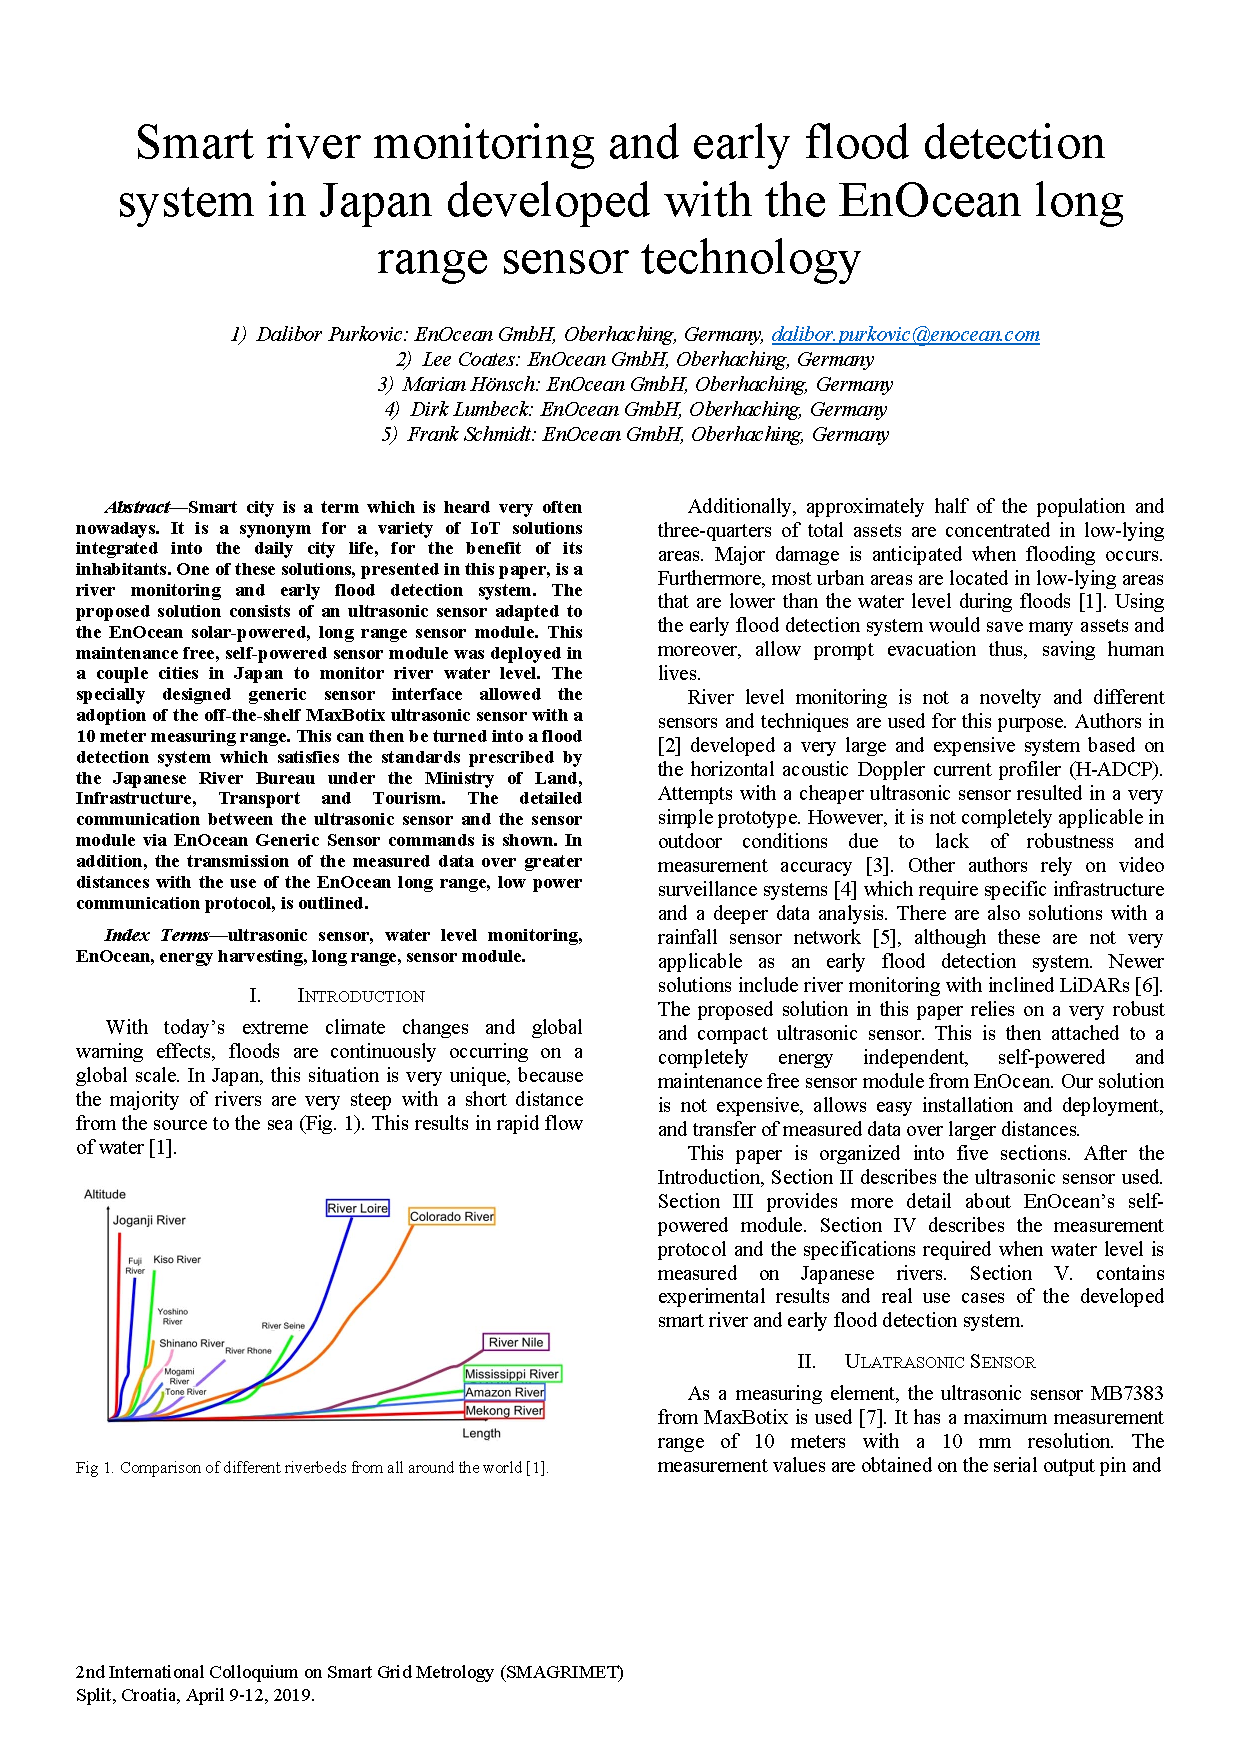
\includepdf[pages=-]{flood2019.pdf}

\begin{thebibliography}{SJL05}
\bibitem{} DIAO YanFang& WANG BenDe ,Risk analysis of flood control operation mode with forecast information based on a combination of risk sources.Sci.China Tech. Sci.MAY 2008.
\bibitem{}Ruan Yun, Vijay P. Singh ,2008, Multiple duration limited water level and dynamic limited water level for flood control, with implications on
water supply. Journal of Hydrology (2008) 354, 160– 170.
\bibitem{} HEIKO APEL, ANNEGRET H. THIEKEN, BRUNO MERZ andGU¨ NTER BLO¨ SCHL,2006, A Probabilistic Modelling System for
Assessing Flood Risks. VOL.12,ISSUE 10.
\bibitem{} Bastian Klein, Ph.D.; Markus Pahlow, Ph.D.;YeshewatesfaHundecha, Ph.D.; and Andreas Schumann, 2005,Probability Analysis of Hydrological
Loads for the Design of Flood Control Systems Using Copulas.J. Hydrol. Eng, vol.15, No.1
 
\bibitem{}  Simon Haykin, Neural Networks – A Comprehiensive Approach.
\bibitem{}  V. Seal, A. Raha, S. Maity, S. Mitra, A. Mukherjee and M. Kanti Naskar,
“A Simple Flood Forecasting Scheme Using Wireless Sensor Networks”,
International Journal of Ad hoc, Sensor & Ubiquitous Computing
(IJASUC) vol. 3, no. 1, February 2012.
\bibitem{}  G. Furquim, F. Neto, G. Pessin, Jo Ueyama, J. P. De Albuquerque, M.
Clara, Eduardo M. Mendiondo, V. C. B. De Souza, P. De Souza, D.
Dimitrova and T. Braun, “Combining Wireless Sensor Networks and
Machine Learning for Flash Flood Nowcasting”, 28th International
Conference on Advanced Information Networking and Applications
Workshops, IEEE, 2014.
\bibitem{}  B. Kontagora Nuhu, T. Arulogun, I. Adeyanju and Abdullahi I.M.,
“Wireless Sensor Network for Real-time Flood Monitoring Based on
6loWPAN Communication Standard”, APTIKOM Journal on Computer
Science and Information Technologies vol. 1, no.1, 2016.

\bibitem{}  S. Gangopadhyay and M. Mondal, “A Wireless Framework for
Environmental Monitoring and Instant Response Alert”, International
Conference on Microelectronics, Computing and Communications
(MicroCom), 23-25 Jan, 2016.
\bibitem{}  P. Mitra, R. Ray, R. Chatterjee, R. Basu, P. Saha, S. Raha, R. Barman, S.
Patra, S. Saha Biswas and S. Saha, “Flood forecasting using Internet of
things and Artificial Neural Networks”, Information Technology,
Electronics and Mobile Communication Conference, IEEE, 2016.
 

\end{thebibliography}
\end{document}


\end{document}